

Узнаем версию системы и проверяем устройства USB

\begin{figure}[h!]
\center{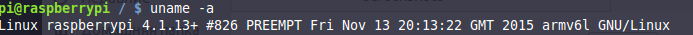
\includegraphics[width=0.6\linewidth]{driver_1}}
\caption{ Узнаем версию системы }
\label{driver_1:driver_1}
\end{figure}


\begin{figure}[h!]
\center{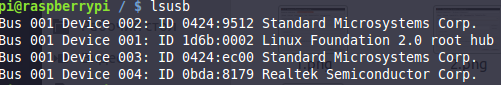
\includegraphics[width=0.6\linewidth]{driver_2}}
\caption{ проверяем устройства USB }
\label{driver_2:driver_2}
\end{figure}


тут ссылка на то,как устанавливать драйвер согласно версии системы
https://www.raspberrypi.org/forums/viewtopic.php?p=462982

Скачиваем драйвер:

\begin{figure}[h!]
\center{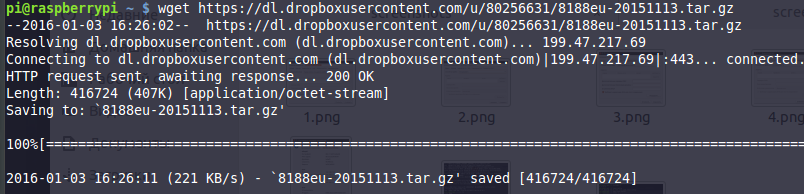
\includegraphics[width=0.6\linewidth]{driver_3}}
\caption{ Скачиваем драйвер }
\label{driver_3:driver_3}
\end{figure}









